\section{Results} \label{ICRA:sec:results}

We begin by describing the two domains for our experiments: bimanual rope manipulation and plant watering. We then validate the claims that (1) our proposed adaptation method achieves lower prediction error in regions of similar dynamics, and (2) that \FOCUS{} achieves higher success rates more quickly in the online adaptation setting compared to baselines which train on all data equally.

\subsection{Bimanual Rope Manipulation}
\label{ICRA:sec:rope}

\begin{figure*}
    \centering
    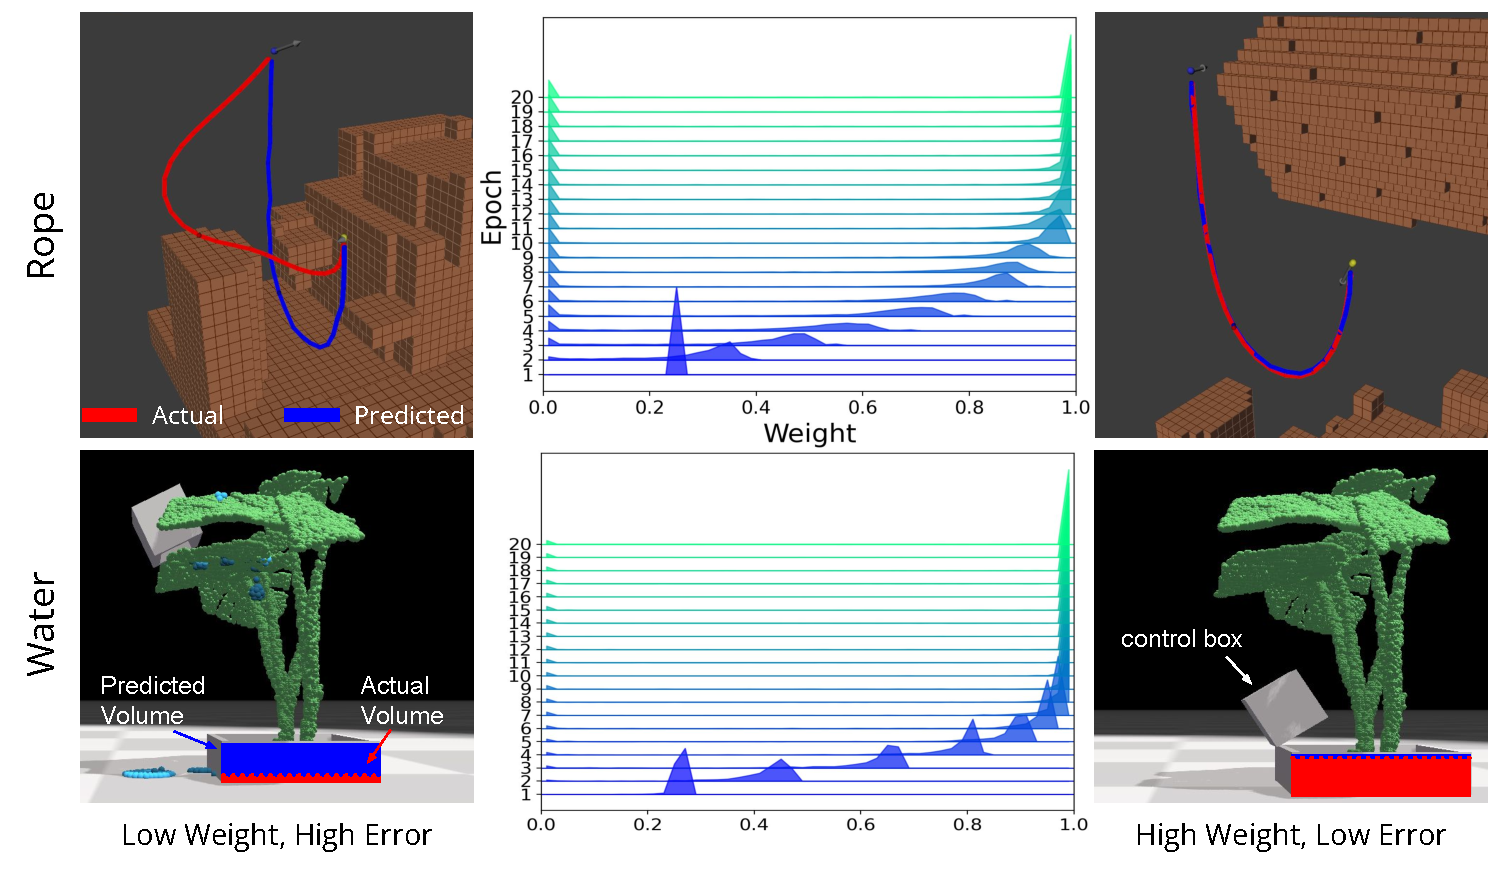
\includegraphics[width=\linewidth]{Chap4/images/data_weight_distribution_figure.pdf}
    \caption{(center) Histograms showing weights assigned to the data according to Equation \eqref{ICRA:eq:adaptation_loss} during the first 20 epochs of training. A histogram is shown for each epoch, where color varies with epoch, and these histograms are staggered along the y-axis. Initially, the weights vary only slightly across the data, but the distribution becomes strongly bimodal as training progresses. Examples of transitions given weight 0 (left) and weight 1 (right) at the end of training.}
    \label{ICRA:fig:weights}
\end{figure*}

In this task, a 16-DOF dual arm robot is holding two ends of a rope in a scene resembling the engine bay of a car (scene shown in Figures \ref{ICRA:fig:real_robot_setup},\ref{ICRA:fig:sim_rope_envs}). The task mimics putting on lifting straps on the engine, which requires moving the rope through narrow passages and around protrusions. The goal is to place the middle of the rope in a goal region defined as a sphere of radius \SI{0.045}{\meter}. The planner outputs gripper position actions, and a local controller executes the actions while maintaining gripper orientations. The learned dynamics model predicts the state of the rope, represented as 25 points, given the initial rope state and gripper position actions.

In the rope manipulation experiments, the source simulation has no obstacles and the robot is simplified to floating kinematic grippers. We then test adaptation to two different target environments: (1) another simulation which includes the robot and obstacles and has different damping and stiffness parameters for the rope, and (2) the real world. Thus, this tests adaptation to a different rope despite the distracting transitions where the rope deforms on the robot or the obstacles. Gazebo with ODE physics is used for simulation \cite{Gazebo}. For rope manipulation, the set $\DST$ would be the transitions from the target environment where the rope is in free space. We use $\softFilteringThrehsold=0.08$.

\subsection{Plant Watering}
\label{ICRA:sec:water}

The goal in this task, illustrated in Figure~\ref{ICRA:fig:waterscene} is to pour at least 75\% of the initial volume from a controlled container into a target container without spilling more than 5\%. The source environment is a variation from the SoftGym PourWater environment~\cite{lin2020softgym}. The target environment has triple the viscosity, a shorter container, and a plant in the target container. Although the agent can pour from above, that causes the water to splatter, which is more difficult to predict than the free-space pours of the target environment. Additionally, the box can collide with the plant, which is dissimilar to the source dynamics where there are no obstacles. The controlled container can rotate about the z-axis The state space is the 4-DOF $[x,y,z,\theta]$ pose of the controlled container, 3-DOF $[x,y,z]$ pose of the target container, control volume, and target volume. The action space is a target pose $[x_{des}, y_{des}, \theta_{des}]$ which is followed by a proportional controller. For plant watering, the set $\DST$ contains free-space motions and pours, whereas collision with and pouring on the plant is not in $\DST$. We use $\softFilteringThrehsold=0.05$.

\subsection{Validating the Adaptation Method}
\label{ICRA:sec:validating_adaptation}

\begin{figure}
    \centering
    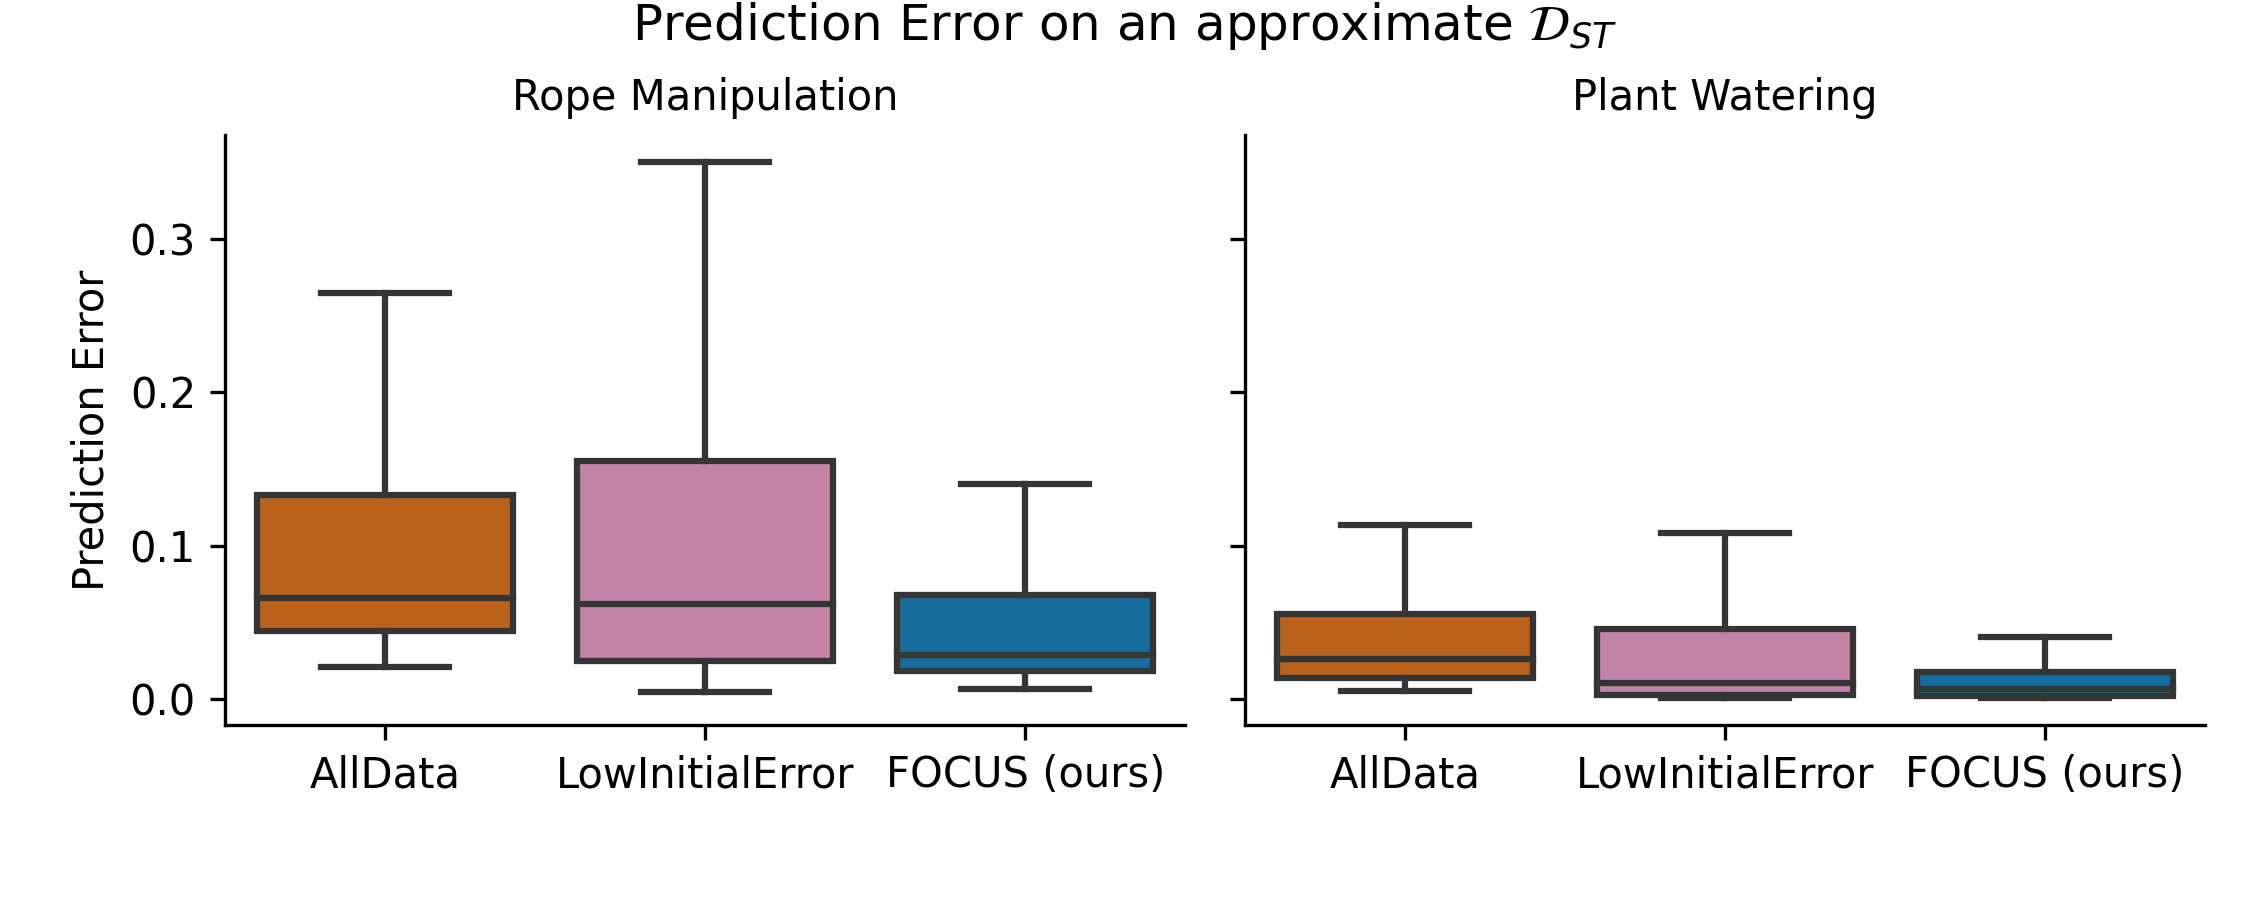
\includegraphics[width=\linewidth]{Chap4/images/known_good_model_error.png}
    \caption{Prediction error for our method versus two baselines, evaluated on a dataset of transitions from regions where the source and target dynamics are similar.}
    \label{ICRA:fig:validating}
\end{figure}

We now evaluate whether the proposed adaptation method achieves lower prediction error on $\DST$. We start by creating validation sets which contain transitions not used for training, and which are known to be in $\DST$. For rope, this means transitions where the rope is in free space. For water, this means transitions which do not collide with or pour over the plant. We evaluate our method and two baselines, all starting from the same pre-trained model and adapting to the same dataset from the target environment. The baseline \textit{AllData} fine-tunes on all transitions with equal weights. The baseline \textit{LowInitialError} uses our weighting function, but computes the weights once using $\learnedDynamics_0$ and does not re-compute them throughout training. Our method uses our proposed loss function (Equation \eqref{ICRA:eq:adaptation_loss}) which re-computes the weights on each batch during training.

For bimanual rope manipulation, the dataset contains 6288 transitions and the validation set contains 792 transitions. For plant watering, the training dataset contains 854 transitions and the validation set contains 130 transitions. The results are visualized in Figure \ref{ICRA:fig:validating}. In both experiments, the error of our method is statistically significantly lower than both baselines ($p<0.0001$).

Figure \ref{ICRA:fig:weights}, demonstrates the intuition behind our adaptation method. In the center, we show histograms over time of the weights assigned to the transitions in the training dataset, for water and for rope. The distribution is initially unimodal since the weighting function when $j=0$ is soft, but as training progresses the distribution rapidly becomes bimodal, where most transitions are given a weight of 1, but some transitions are given a weight of 0. We show examples of these low and high weight transitions on either side. For rope manipulation, we found that the number of the transitions with prediction error below $\gamma$ increases from 52\% at epoch 1 to 80\% at epoch 20, which shows that the subset of data we train on grows. This explains why our method outperforms the \textit{LowInitialError} baseline, since that baseline is not making use of as much of the data as our method does. The presence of transitions with 0 weight (e.g. 20\% for rope at epoch 20) shows that our method is not converging to training on all examples, which does not perform well based on the \textit{AllData} baseline.

\subsection{Online Learning Experiments}
\label{ICRA:sec:online_learning_experiments}

\begin{figure*}
     \centering
     \begin{subfigure}[b]{0.32\textwidth}
         \centering
         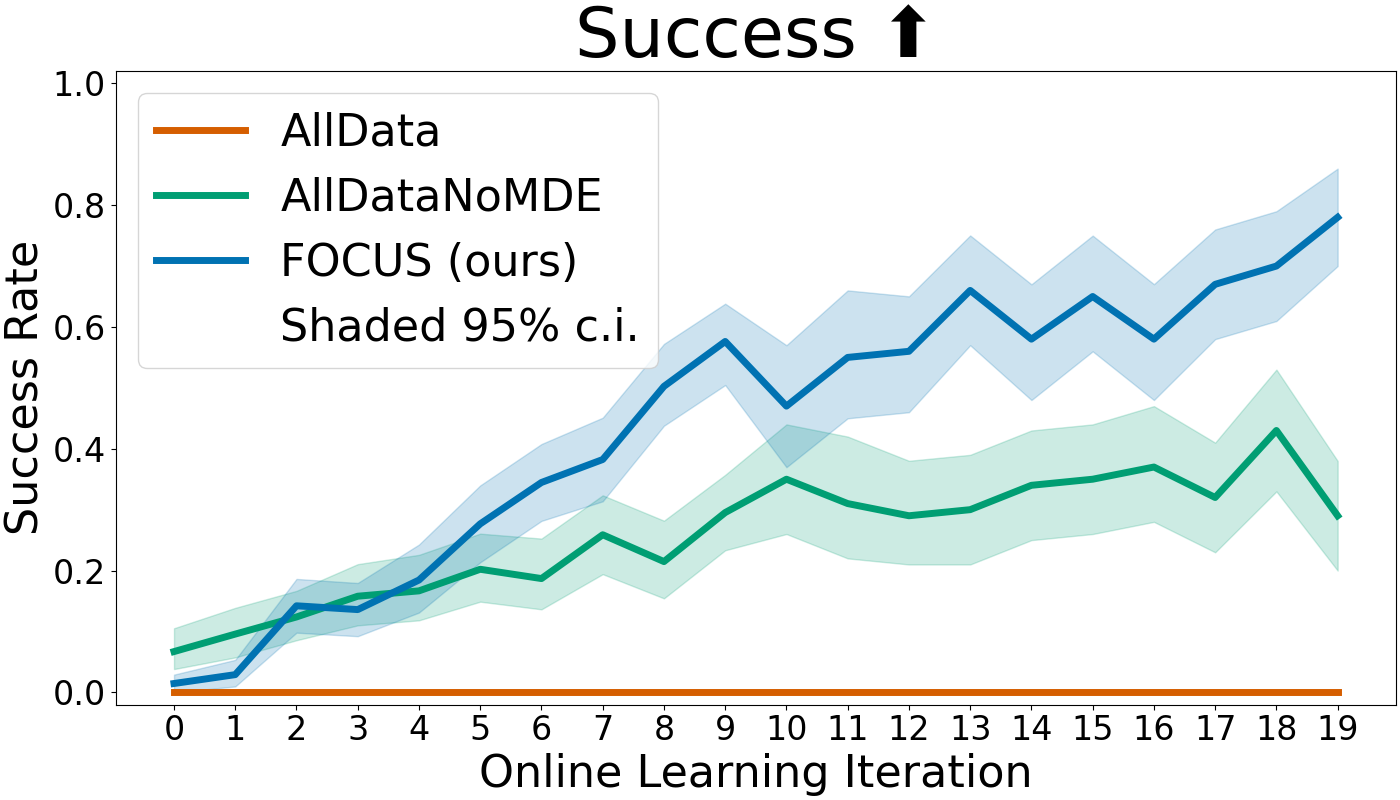
\includegraphics[width=\linewidth]{Chap4/images/success.png}
     \end{subfigure}
     \hfill
     \begin{subfigure}[b]{0.32\textwidth}
         \centering
         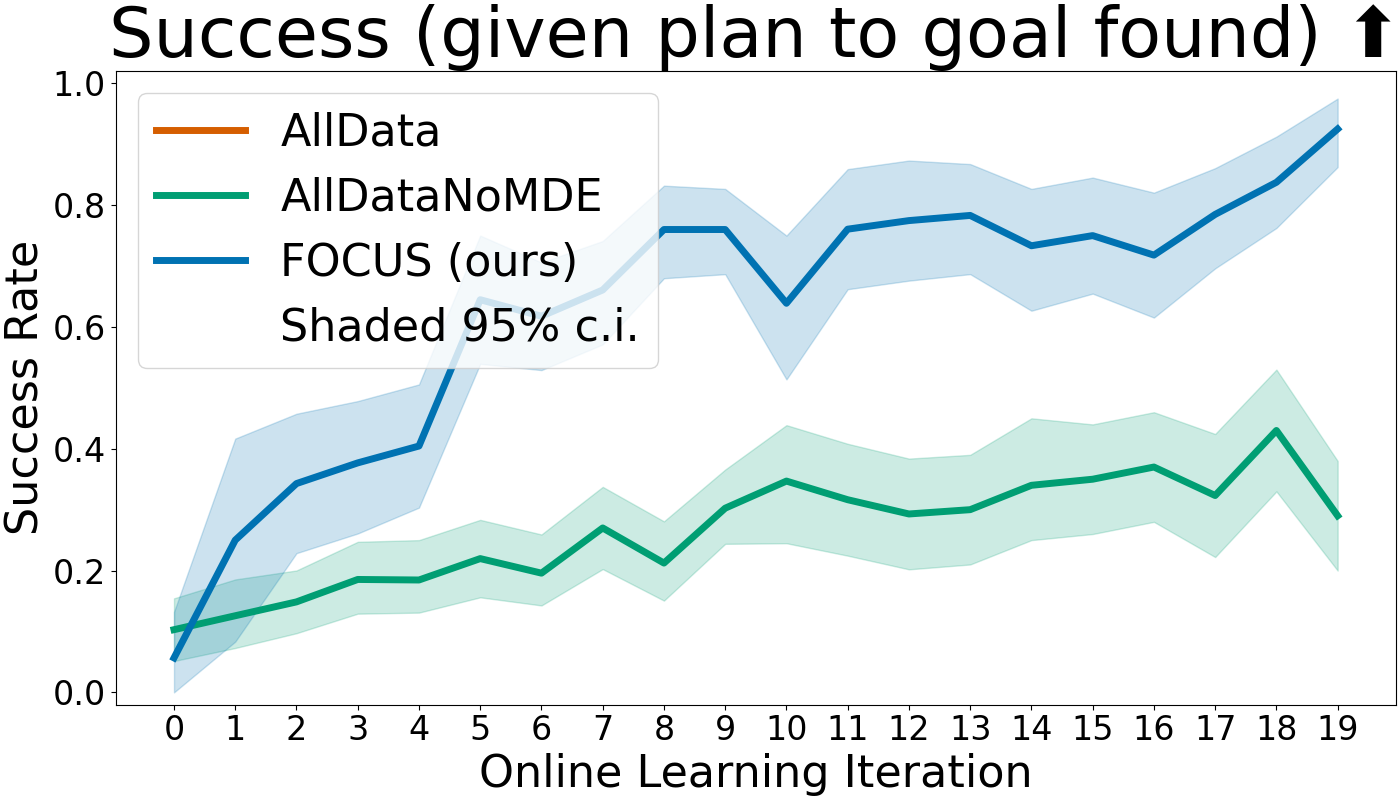
\includegraphics[width=\linewidth]{Chap4/images/success_given_plan_found.png} 
     \end{subfigure}
     \hfill
     \begin{subfigure}[b]{0.32\textwidth}
         \centering
         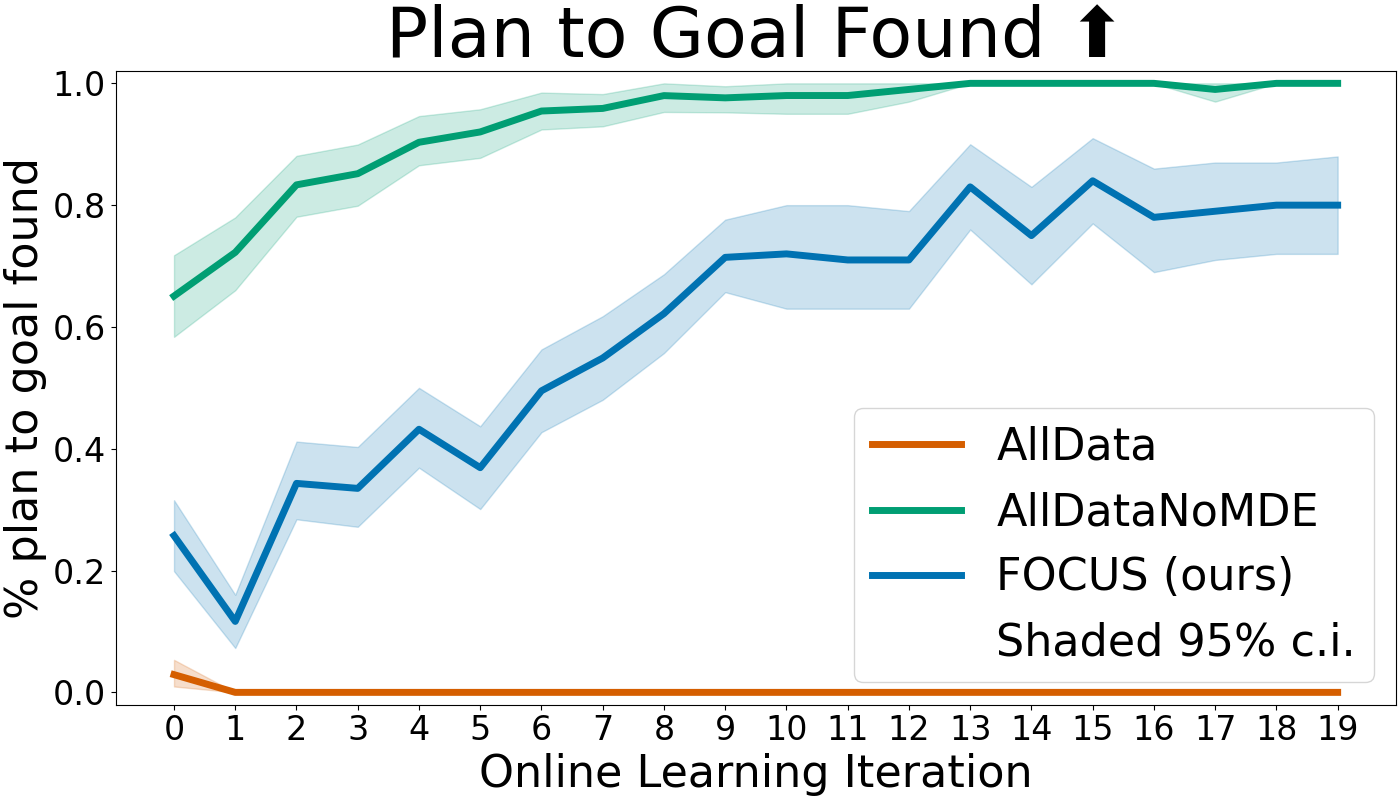
\includegraphics[width=\linewidth]{Chap4/images/plan_found.png}
     \end{subfigure}
    \caption{Post-learning evaluation of rope manipulation in simulation: Three metrics shown over the 20 iterations of online learning. The shaded interval is the 95\% confidence interval, with the boot-strapping method used by Seaborn.}
    \label{ICRA:fig:sim_rope_results}
\end{figure*}

We show that \FOCUS{} achieves higher task success with fewer data than baselines which fine-tune the dynamics on all available data. The first baseline, called \textit{AllDataNoMDE} does not use our proposed adaptation method and does not use MDEs when planning, which makes it a conventional online learning method. The second, called \textit{AllData} includes MDEs in planning, but ablates our fine-tuning method. First, we evaluate in the rope manipulation domain on adaptation from one simulation to another (see Figure \ref{ICRA:fig:sim_rope_envs}). We ran 20 iterations of online learning, where each iteration consists of 10 episodes, which amounts to roughly $6,000$ transitions in total during learning. We then repeated this 10 times for each method/baseline with different random seeds.

After learning, we took the models saved after each learning iteration and ran 100 episodes of evaluation per method. To maximize success rates of all methods, we use a longer timeout and do not allow random-accepts when planning. We also stop execution and replan if the error between the plan and the observed state exceeds a large threshold on model error (0.25).

The results of this first experiment are summarized in Figure \ref{ICRA:fig:sim_rope_results}. The proposed method (\FOCUS{}) shows the highest success rate when plans are found. The \textit{AllData} method, which ablates our method for fine-tuning the dynamics, never finds paths to the goal. This is because its dynamics are not sufficiently accurate, and so the MDE constraint makes the planning problem infeasible. Accurately learning the dynamics in the \textit{AllData} or \textit{AllDataNoMDE} methods would involve predicting the deformation of the rope on obstacles, which is challenging given a dataset of only a few thousand transitions.

\begin{figure}
    \centering
    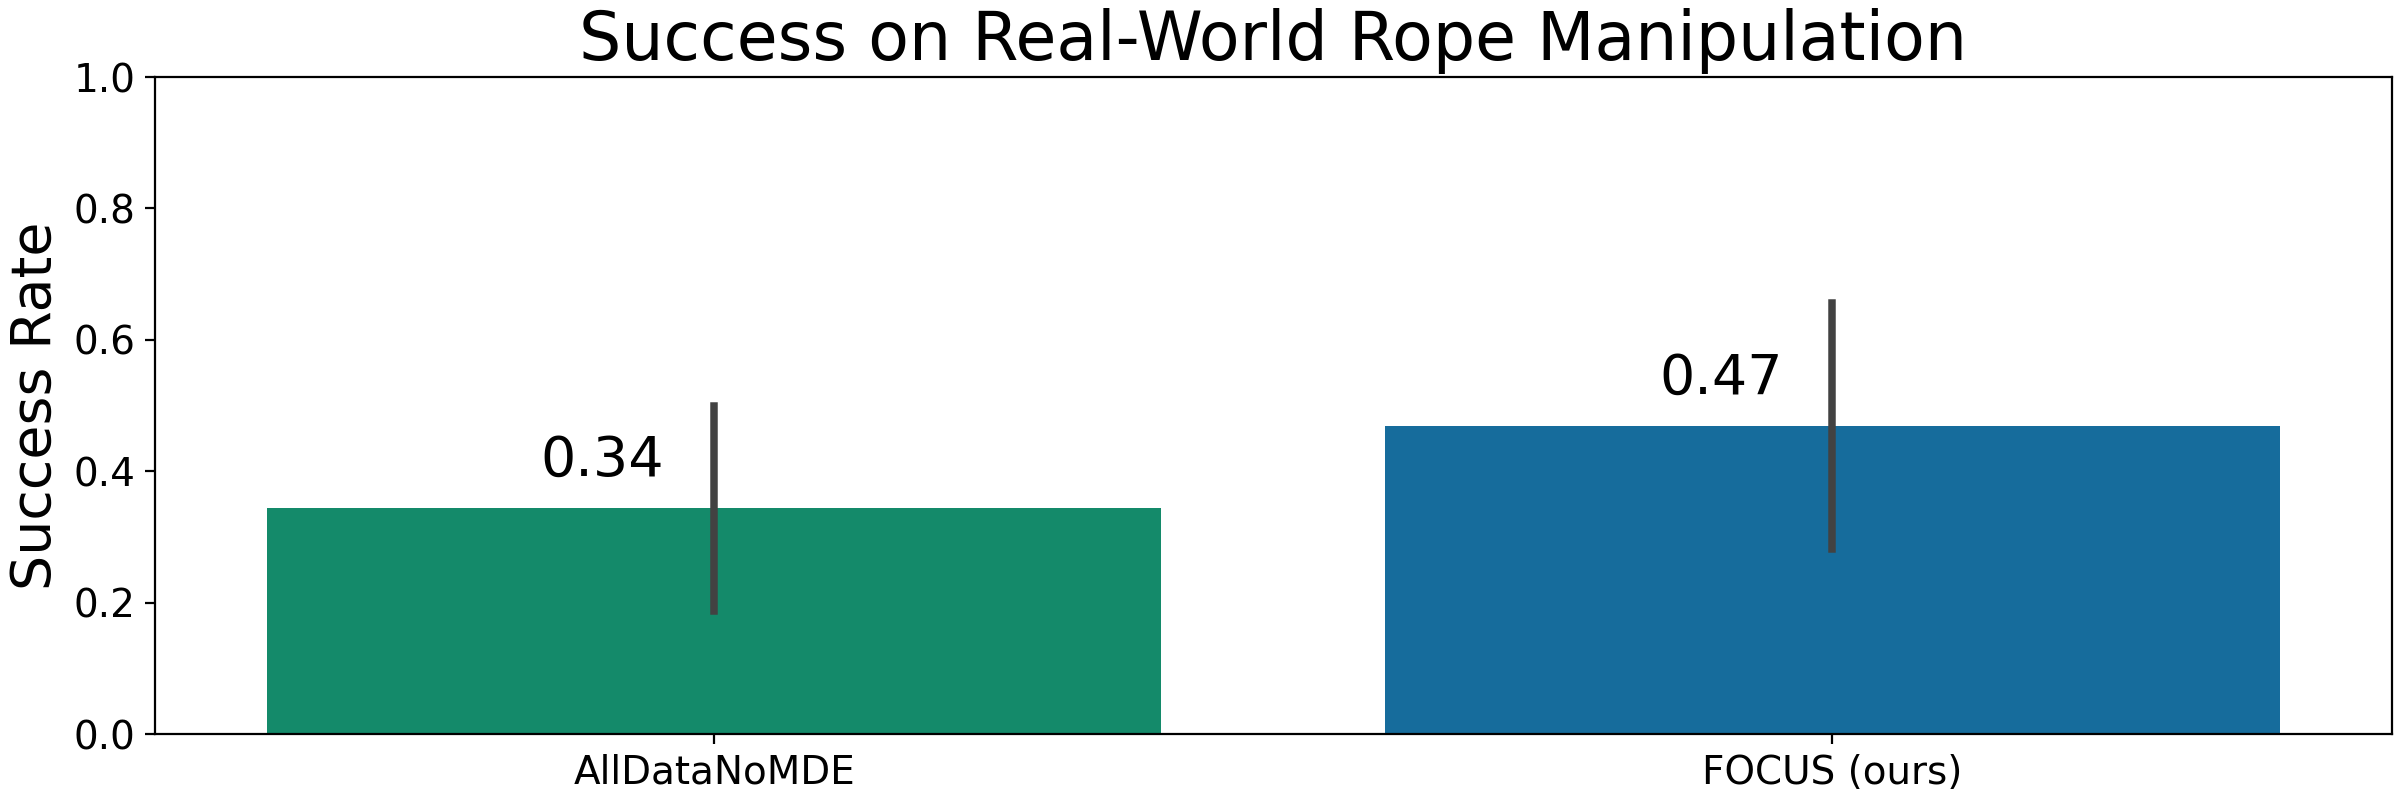
\includegraphics[width=0.7\linewidth]{Chap4/images/real_success.png}
    \caption{Success rate for the \textit{AllDataNoMDE} baseline (left) versus \FOCUS{} (right) for online adaptation to real world bimanual rope manipulation.}
    \label{ICRA:fig:real_rope_success}
\end{figure}

\subsection{Real Robot Results}

We performed a similar experiment to the first rope manipulation experiment, but on real robot hardware where sensor and actuator noise are substantial factors (approximately \SI{5}{\centi\meter} of end-effector error). More importantly, it demonstrates how \FOCUS{} enables a robot to quickly learn a task in the real world. We use CDCPD2 \cite{CDCPD2} to track the rope state. The geometry of the car scene is approximated with primitive geometric shapes. We use the same source simulation environment as for the  simulation rope experiment, but now the target environment is the real world. The robot must learn to adapt the simulated free-space rope dynamics to the real world, despite the different real-world free-space dynamics and the fact that the rope can deform on the robots' arms or on the objects in the scene. Because perception and actuation error are higher in the real world than in simulation, we use $\softFilteringThrehsold=0.2$.

We ran the online learning procedure with a single start configuration and a single goal region for one random seed and compare \FOCUS{} to the \textit{AllDataNoMDE} baseline, since \textit{AllDataNoMDE} performed best in simulation. After 15 iterations of learning, we freeze the models and evaluate task success 32 times. The success rates are shown in Figure \ref{ICRA:fig:real_rope_success}. With \FOCUS{}, the robot successfully placed the rope under the engine 15/32 times, while \textit{AllDataNoMDE} succeeded 11/32 times. Achieving high success rates in this task is difficult due to narrow passages, perception error, and actuator error. Failure modes for FOCUS include the rope getting pulled out of the robots' hands, getting too close and catching on obstacles, and failing to find plans that reach the goal.
